% Generado por analysis/src/tablas/figuras_tex.py — no editar a mano.
\begin{figure*}[!tbp]
\centering
\begin{minipage}[b]{0.56\textwidth}\centering
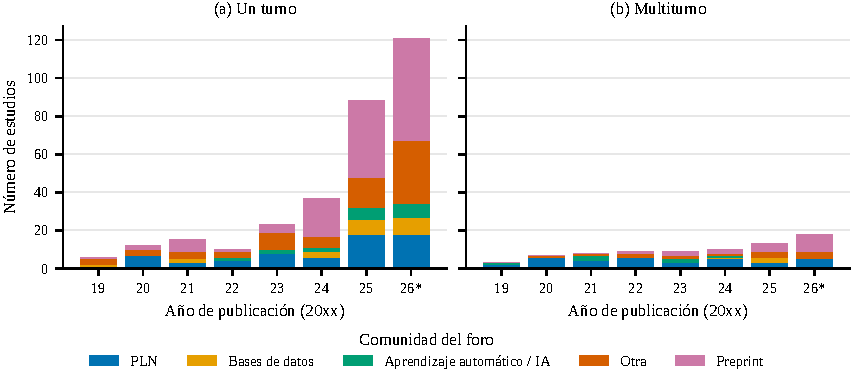
\includegraphics[width=\linewidth]{bib_comunidad}\\(a)\\[3pt]
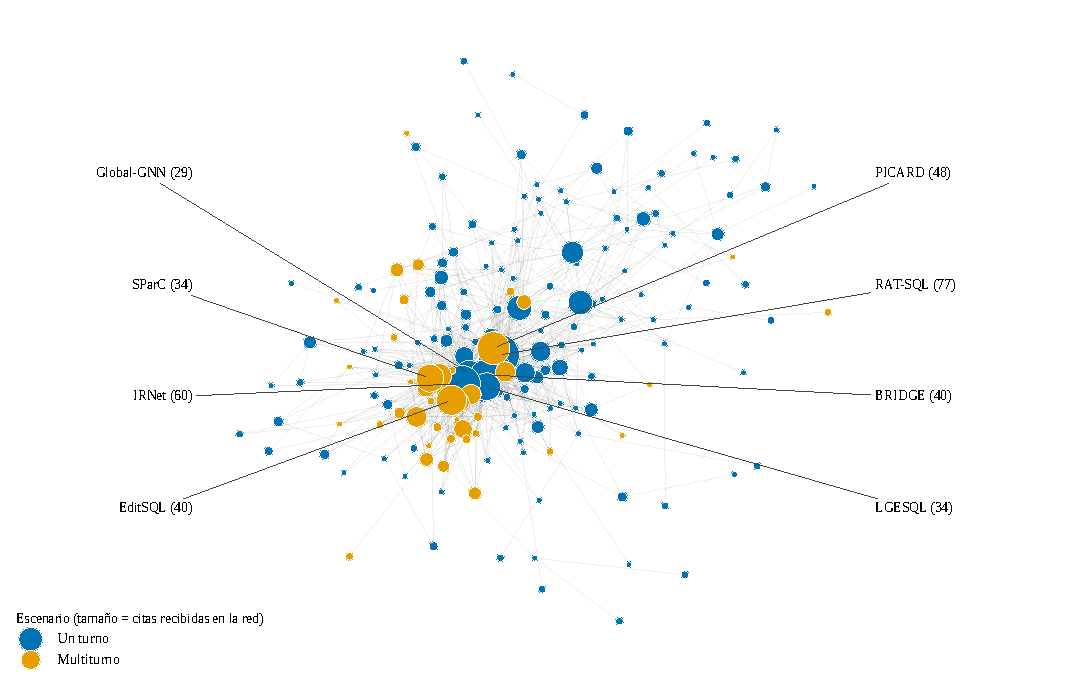
\includegraphics[width=\linewidth]{bib_red_citas}\\(b)
\end{minipage}\hfill
\begin{minipage}[b]{0.42\textwidth}\centering
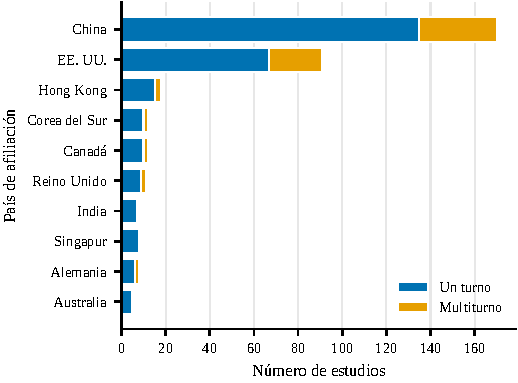
\includegraphics[width=0.82\linewidth]{bib_paises}\\(c)\\[3pt]
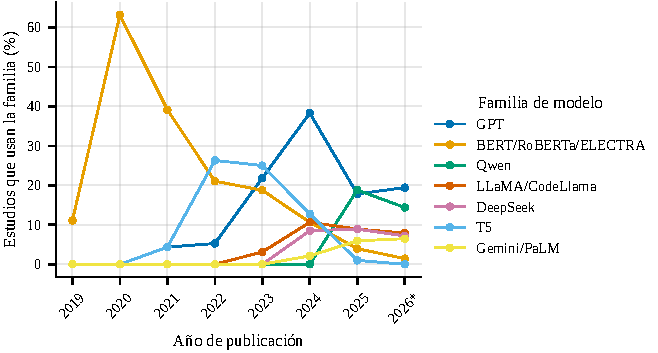
\includegraphics[width=\linewidth]{bib_modelos}\\(d)
\end{minipage}
\caption{Panorama bibliométrico exploratorio (enmienda A6). (a) Comunidad de investigación del foro de publicación, por año: (a) estudios de un turno; (b) estudios multiturno. *2026: año parcial. (b) Red de citas entre los estudios incluidos con al menos un vínculo (184 de 389 estudios; 841 citas; fuente: OpenAlex, 2026-10-13). Etiquetas: los ocho estudios más citados dentro de la red, con su número de citas. (c) Los diez países con más estudios incluidos, por escenario. Un estudio se cuenta en cada país con al menos un autor afiliado (fuente: OpenAlex, 2026-10-13). (d) Familias de modelos base por año (porcentaje de los estudios del año que mencionan la familia; un estudio puede usar varias). En el Nivel 1 solo se registraron los modelos citados en las páginas 1–2, por lo que el uso real está subestimado. *2026: año parcial.}
\label{fig:bib_panorama}
\end{figure*}
